\section{Introduzione}

Un riflesso fisiologico è una risposta involontaria ad un stimolo, mediata da elementi del sistema nervoso. Generalmente lo scopo dei riflessi fisiologici è quello di mantenere l'omeostasi dell'organismo ed evitare situazioni di pericolo, mantenendo al sicuro l'organismo stesso.

Generalmente, per parlare di riflesso, si parte dallo stimolo caratterizzandolo al cambiamento di una variabile ambientale o alla variazione di un particolare segnale. Tale stimolo viene sentito da un sensore, in fisiologia un recettore sensoriale, che si occupa di monitorare l'ambiente interno ed esterno all'organismo.

Dal recettore parte la via afferente verso i centri di integrazione dove lo stimolo viene elaborato, in maniera più o meno complessa, elaborandone una risposta che, tramite una via efferente, verrà trasmessa all'effettore.

Tra i riflessi fisiologici dell'organismo umano spiccano il riflesso da stiramento muscolare e il riflesso pupillare. Tali riflessi si differenziano nello stimolo inducente ma sono accomunati da avere come risposta la contrazione o il rilassamento di fibre muscolari. 

Si possono studiare tali riflessi modellandoli e analizzandoli con le teorie dei controlli automatici per osservarne come variazioni nel guadagno del riflesso , ad esempio dovute a patologie fortemente debilitanti, portano ad instabilità in entrambi i sistemi.

Nel seguente report vengono propositi due differenti modelli e la loro implementazione nell'ambiente Simulink, analizzandone il comportamento.

\section{Background}


\begin{figure*}[t!]
	\centering
	\begin{subfigure}{0.33\linewidth}
		\centering
		\footnotesize{\def\svgwidth{0.9\linewidth}
			\input{modello_muscolo_schema.pdf_tex}}
		\caption{}
		\label{fig:hill}
	\end{subfigure}\hfill
	\begin{subfigure}{0.33\linewidth}
		\centering
		\tiny{\def\svgwidth{0.8\linewidth}
			\input{fuso_modello.pdf_tex}}
		\caption{}
	\end{subfigure}\hfill
	\begin{subfigure}{0.33\linewidth}
		\centering
		\footnotesize{\def\svgwidth{0.9\linewidth}
			\input{modello_fuso_schema.pdf_tex}}
		\caption{}
		\label{fig:soecthing}
	\end{subfigure}\hfill
	\caption{Modello muscolare di Hill (a); relazione tra muscolo e fuso neuromuscolare (b); modello di fuso neuromuscolare di Soechting (c) dove si distinguono le rigidezze polari $K_{sp}$ e del nucleo $K_{ss}$.}
	\label{fig:fuso}
\end{figure*}


Un sistema di controllo è un apparato che consente di manipolare il comportamento del sistema da controllare in relazione ad un'evoluzione temporale delle grandezze di ingresso. Ovvero, un insieme di componenti interconnessi che lavorano per raggiungere una determinata risposta anche in presenza di stimoli esterni \cite{marro_controlli_2004}.  

Si parla di regolazione, o controllo semplice, quando si richiede che l'uscita rimanga costante al variare dell'ingresso.

Ove possibile si utilizzano sistemi di controllo ad anello chiuso dove si identifica anche il blocco di retroazione che genera un segnale proporzione al valore della grandezza controllata, riportandolo in ingresso al controllore.

All'interno degli organismi biologici si trovano diversi sistemi di controllo, più o meno complessi, alcuni locali e altri diffusi su tutto l'organismo, volti a mantenere l'omeostasi dell'organismo. 

Il termine omeostasi fu introdotto nel 1865 da Claude Bernard per rappresentare come l'organismo cercasse di mantenere costante l'ambiente interno del corpo \cite{bernard1957introduction}. Il termine fu poi coniato da Walter Bradford Cannon, ampliandone il significato e introducendo il fatto che l'omeostasi non è uno stato statico stazionario ma è un proprio un continuo evolversi di stati di equilibrio e di condizioni che possono continuamente variare \cite{cannon1939wisdom}. Questo è dovuto all'elevata complessità dei sistemi di controllo fisiologici che coinvolgono sicuramente il sistema nervoso ma anche i singoli organi. 

Quindi, l'estensione del concetto di omeostasi può essere visto come l'oscillazione nel tempo intorno ad un valore medio caratteristico di ogni variabile fisiologica. Tale oscillazione nel tempo può essere riferita a secondi, minuti, giorni, ore o anni a secondi di quale parametro si considera. Tuttavia, trascorriamo la maggior parte del tempo oscillando tra un valore massimo e minimo, attorno al valore medio, in un range considerato normale. Tale range è proprio ciò che viene definito omeostasi \cite{davies_adaptive_2016}. 

\subsection{Riflesso neuromuscolare}



Quando un muscolo intero viene stirato passivamente le fibre del fuso neuromuscolare si stirano e aumentano la frequenza di scarica nelle fibre nervose afferenti. Le loro terminazioni sensoriali, che terminano sulle fibre intrafusali stirate, sono tali per cui il neurone afferente stabilisce contatti sinaptici direttamente sul motoneurone $\alpha$ che innerva le fibre extrafusali dello stesso muscolo. L'attivazione di questo contatto sinaptico determina la contrazione del muscolo che risultava eccessivamente stirato.

Questo riflesso miotatico funge da meccanismo locale a feedback negativo che permette di opporsi ad ogni variazione passiva della lunghezza muscolare, così da mantenere la lunghezza di stiramento ottimale. 

Ne sono esempi il riflesso rotuleo o il riflesso da stiramento nel braccio, entrambi usati anche come test clinico di routine per valutare il sistema nervoso. 

Tali riflessi possono essere assenti o depressi a causa di perdite di input eccitatori dai livelli superiori o per perdite di input inibitori ai motoneuroni dai livelli encefalici superiori \cite{sherwood_fisiologia_2008}.

Questo riflesso coinvolge il muscolo stesso, il fuso neuromuscolare e i motoneuroni. Tali partecipanti possono essere rivisti come un sistema di controllo. 

Concentrandoci sull'arto superiore è possibile vedere il centro del riflesso nel midollo spinale, dove avviene la sinapsi tra le vie afferenti e i motoneuroni $\alpha$ per regolare il muscolo a seconda del disturbo indotto dal carico.


Affinché sia possibile analizzare i singoli sistemi è necessario adottare un modello matematico descrittivo.

Partendo dalla descrizione geometrica in \cref{fig:avambraccio} il sistema è descritto dalla seguente equazione:

\begin{equation}
	M_{x}(t)-M(t)=J \ddot{\theta}
\end{equation}



\begin{figure*}[t!]
	\centering
	\begin{subfigure}{0.7\linewidth}
		\centering
		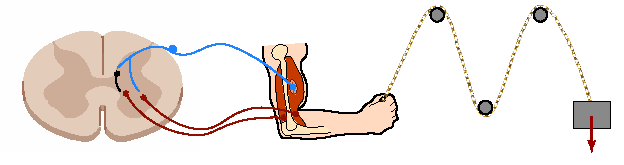
\includegraphics[width=0.95\linewidth]{figures/avambraccio_schema}\caption{}
	\end{subfigure}\hfill
	\begin{subfigure}{0.3\linewidth}
		\centering
		\footnotesize{\def\svgwidth{0.9\linewidth}
			\input{avambraccio_modello.pdf_tex}}
		\caption{}
	\end{subfigure}
	\caption{Rappresentazione schematica del test diagnostico per il riflesso da stiramento del braccio (a). Il carico viene applicato tramite una carrucola e va stimolare i recettori del fuso neuromuscolare che a loro volta vanno a stimolare i percorsi delle vie riflesse all'interno del canale spinale; gradi di libertà del sistema braccio-avambraccio (b) dove la coppia è esercitata dal muscolo}
	\label{fig:avambraccio}
\end{figure*}





\subsubsection{Modello di muscolo}

Viene considerato il modello di muscolo di Hill \cite{hill_heat_1938}. Tale modello, a parametri concentrati, considera il muscolo come la serie di due zone. La prima zona è data da un parallelo di una coppia motrice (forza muscolare) e uno smorzamento, ed è a sua volta in serie ad una rigidezza elastica (\cref{fig:hill}).

Mentre lo spostamento angolare sarà la somma dei due blocchi, la coppia risultante sarà uguale nel parallelo:

\begin{equation}
	\begin{gathered}
		M(t)=K\left(\theta-\theta_{1}\right) \\
		M(t)=M_{0}(t)+B \dot{\theta}_{1}
	\end{gathered}
\end{equation}

Quindi, derivando la prima e sostituendo $\theta_1$ nella seconda, può essere descritto dinamicamente dalla seguente equazione:

\begin{equation}
	M_{x}(t)-M_{0}(t)=\frac{B J}{K} \dddot{\theta}(t)+J \ddot{\theta}(t)+B \dot{\theta}(t)
\end{equation}

E, nel dominio di Laplace, da:

\begin{equation}
	M_{x}(s)-M_{0}(s)=s\left(\frac{B J}{k} s^{2}+J s+B\right)\theta (s)
\end{equation}

\subsubsection{Fuso neuromuscolare}

\begin{figure}[t!]
	\centering
	\footnotesize{\def\svgwidth{0.95\linewidth}
		\input{blocchi_stretch.pdf_tex}}
	\caption{Diagramma a blocchi del riflesso neuromuscolare. Si possono distinguere il sotto-sistema muscolare (in blu) e il sotto-sistema del riflesso vero e proprio (in verde)}
	\label{fig:sistemamuscolo}
\end{figure}

\begin{table}[t!]
	\centering
	\begin{tabular}{|c|c|}
		\hline
		Parametro & Valore \\
		\hline
		\texttt{B} & 2 [Nms] \\
		\hline
		\texttt{J} & 0.1 [kg m\textsuperscript{2}] \\
		\hline
		\texttt{Td} & 0.02 [s] \\
		\hline
		\texttt{beta} & 100 \\
		\hline
		\texttt{eta} & 5 \\
		\hline
		\texttt{k} & 50 [Nm] \\
		\hline
		\texttt{tau} & 1/300 [s] \\
		\hline
	\end{tabular}
	\caption{Parametri del sistema descrittivo del riflesso neuromuscolare}
	\label{tab:parametriMuscolo}
\end{table}


Per il fuso muscolare viene adottare il modello di Soechting \cite{mains_model_1971} dove il fuso viene differenziato tra la parte interna, del nucleo, e la parte polare. Si considera la serie di una zona data dal parallelo di una rigidezza elastica e uno smorzatore viscoso con una seconda rigidezza elastica (\cref{fig:soecthing}).

La variabile di interesse è sempre la coordinata angolare e valgono le seguenti relazioni:

\begin{equation}
	\begin{gathered}
		M_{s}(t)=K_{s s}\left(\theta-\theta_{2}\right) \\
		M_{s}(t)=K_{s p}  \theta_{2}+B_{s} \dot{\theta}_{2}
	\end{gathered}
\end{equation}

\subsubsection{Riflesso}

\begin{figure*}[t!]
	\centering
	\begin{subfigure}{0.6\linewidth}
		\centering
		\tiny{\def\svgwidth{0.95\linewidth}
			\input{occhio_muscoli.pdf_tex}}
		\caption{}
	\end{subfigure}\hfill
	\begin{subfigure}{0.4\linewidth}
		\centering
		\tiny{\def\svgwidth{0.95\linewidth}
			\input{circuito_pupilla.pdf_tex}}
		\caption{}
	\end{subfigure}
	\caption{Lo stroma dell'iride contiene uno strato di tessuto connettivo ricco di cellule muscolare lisce (a). Uno strato, a forma di anello, forma il muscolo costrittore, o sfintere pupillare, mentre nella faccia posteriore è presente il muscolo dilatatore della pupilla con le fibre disposte radialmente. Il sistema di controllo del riflesso pupillare (b) volto a restringere e dilatare la pupilla, tramite le vie superiori, a seconda del flusso luminoso incidente sulla retina}
	\label{fig:pupilla}
\end{figure*}

Per il riflesso sappiamo che conta quanto accade a livello del fuso, ovvero avremo la risposta legata all'allungamento per il tramite di un certo guadagno:

\begin{equation}
	M_{0}(t)=\beta\left(\theta-\theta_{2}\right)
\end{equation}

Da cui si trova l'equazione del sistema:

\begin{equation}
	\small{\dot{M}_{0}(t)+\frac{M_{0}(t)}{\tau}=\beta\left(\dot{\theta}\left(t-T_{D}\right)+\frac{\theta\left(t-T_{D}\right)}{\tau \eta}\right)}
\end{equation}

Dove i due parametri, funzioni delle costanti concentrate, sono:

\begin{equation}
	\tau=\frac{B_{s}}{K_{s s}+K_{s p}} \quad \text { e } \eta=\frac{K_{s s}+K_{s p}}{K_{s p}}
\end{equation}

Passando nel dominio di Laplace possiamo ricavare la coppia agente come:

\begin{equation}
	M_{o}(s)=\beta\left(\frac{s \tau+s / \eta}{s \tau+s}\right) e^{-s T_{D}} \theta(s)
\end{equation}

Per l'implementazione in Simulink vengono considerati dei parametri fisiologici noti in letteratura \cite{khoo_physiological_2018,soechting_evaluation_1971}, in \cref{tab:parametriMuscolo} . 

Tale sistema può essere rappresentato in un diagramma a blocchi, tipico dei controlli automatici, raffigurato in \cref{fig:sistemamuscolo}.



\subsection{Riflesso fotomotore}


Un altro riflesso di grande interesse clinico è il riflesso pupillare, noto anche come riflesso fotomotore. Tale riflesso controlla il diametro della pupilla in risposta all'intensità della luce che arriva alla retina.

Il nervo ottico costituisce la via afferente in quanto percepisce la luce in ingresso, tramite  le cellule gangliari della retina. L'informazione raggiunge il nucleo pretettale nel mesencefalo superiore e poi il nucleo di Edinger-Westphal. Da qui si dipartono i nervi oculomotori fino ai gangli ciliari e all'invervazione del muscolo costrittore della pupilla \cite{kandel_principles_2021}.

In condizioni fisiologiche, le pupille rispondono entrambe in maniera identica. Il confronto delle risposte asimmetriche permette di valutare una lesione.
Ad esempio, una risposta diretta in una pupilla senza risposta consensuale nell'altra indica un possibile problema nella connessione motoria della seconda. Oppure, è possibile avere perdite del riflesso diretto mentre rimane attiva la risposta consensuale. 

\subsubsection{Modello di Stark}

\begin{table}[t!]
	\centering
	\begin{tabular}{|c|c|}
		\hline
		Parametro & Valore \\
		\hline
		\texttt{K} & 0.16 \\
		\hline
		\texttt{D} & 0.18 [s] \\
		\hline
		\texttt{tau} & 0.1 [s] \\
		\hline
	\end{tabular}
	\caption{Parametri del sistema linearizzato descrittivo del riflesso pupillare}
	\label{tab:pupilla}
\end{table}



\begin{figure}[t!]
	\centering
	\footnotesize{\def\svgwidth{0.95\linewidth}
		\input{blocchi_pupillary.pdf_tex}}
	\caption{Diagramma a blocchi del riflesso pupillare linearizzato}
	\label{fig:pupillary_block}
\end{figure}

Per l'implementazione viene considerato il modello di Stark \cite{stark_servoanalytic_1957}. Tale modello interpreta il flusso di luce come l'intensità luminosa agente sull'area della pupilla e l'obiettivo del controllore (riflesso pupillare) è proprio quello di mantenere tale flusso costante. Se varia il flusso il sistema nervoso si attiva per variare l'area della pupilla.

Tale modello contiene molte non linearità ma, linerizzandolo intorno al punto di lavoro, permette di descrivere adeguatamente la risposta fisiologica \cite{khoo_physiological_2018}.

Il diagramma a blocchi del sistema è presente in \cref{fig:pupilla}. Si considera quindi un sistema LTI con una funzione di trasferimento del terzo ordine in serie ad un ritardo con costante di tempo $\tau$. Tale sistema è stato descritto da Stark in seguito ad un'accurato fitting dei dati sperimentali.

Ovvero la funzione di trasferimento di anello :

\begin{equation}
	H(s)=\frac{K e^{-s D}}{(1+\tau s)^{3}}
\end{equation}

Dove il guadagno è dato dal prodotto del guadagno della funzione di trasferimento del cambiamento d'area e del fattore linearizzato di intensità luminosa (rispetto al quale si è linearizzato il modello), ovvero:

\begin{equation}
	K=I_{\text {ref }} K_{1}
\end{equation}

I parametri del sistema sono presenti in \cref{tab:pupilla}.



\subsection{Stabilità}

Per un sistema dinamico uno stato di equilibrio è uno stato in cui il sistema rimane indefinitamente, in assenza di perturbazioni. Se tale stato di equilibrio è stabile (asintoticamente), ciò permette al sistema di rimanerci effettivamente. 

Per un sistema lineare si può parlare di stabilità del sistema stesso (e non solo del punto di equilibrio) ed in particolare risulta stabile qualora gli autovalori della matrice dinamica del sistema sono a parte reale negativa \cite{grasselli_sistemi_2008}.

Tale definizione matematica può essere particolarizzata in diversi criteri per analizzare la stabilità del singolo sistema.

Considerando un generico sistema a retroazione di equazione caratteristica:

\begin{equation}
	1+G(s)H(s)=0
			\label{eq:retroazione}
\end{equation}

Dove $G(s)$ è la funzione di trasferimento diretta e $H(s)$ la funzione di trasferimento di retroazione e $G(s)H(s)$ la funzione di trasferimento di anello (\cref{fig:sistema}).

Quindi tale per cui:

\begin{equation}
	Y(1+G H)=G X
\end{equation}

E allora la funzione di trasferimento:

\begin{equation}
	W=\frac{Y}{X}=\frac{G}{1+G H}
\end{equation}


\begin{figure}[t!]
	\centering
	\centering
\footnotesize{\def\svgwidth{0.95\linewidth}
	\input{feedback.pdf_tex}}
	\caption{Generico sistema a feedback negativo dove sono presenti la funzione di trasferimento diretta $G(s)$ e la retroazione $H(s)$ che riporta l'uscita in ingresso con segno invertito}
	\label{fig:sistema}
\end{figure}


Considerando che $G(s)H(s)$ è una funzione razionale fratta con guadagno $K$ (positivo per sistemi a retroazione negativa), le radici di tale equazione descrivono una curva nel piano $s$ che prende il nome di luogo delle radici. 

\begin{equation}
	G(s)H(s)=K\left.N(s)\over D(s)\right.
\end{equation}

Per avere stabilità si richiede che tutti i poli della funzione di trasferimento siano nella parte sinistra del piano, ovvero a parte reale negativa \cite{marro_controlli_2004}. Tali poli corrispondono agli zeri di \cref{eq:retroazione} ovvero a studiare l'andamento:

\begin{equation}
D(s)+KN(s)=0
\end{equation}


\begin{figure*}[t!]
	\centering
	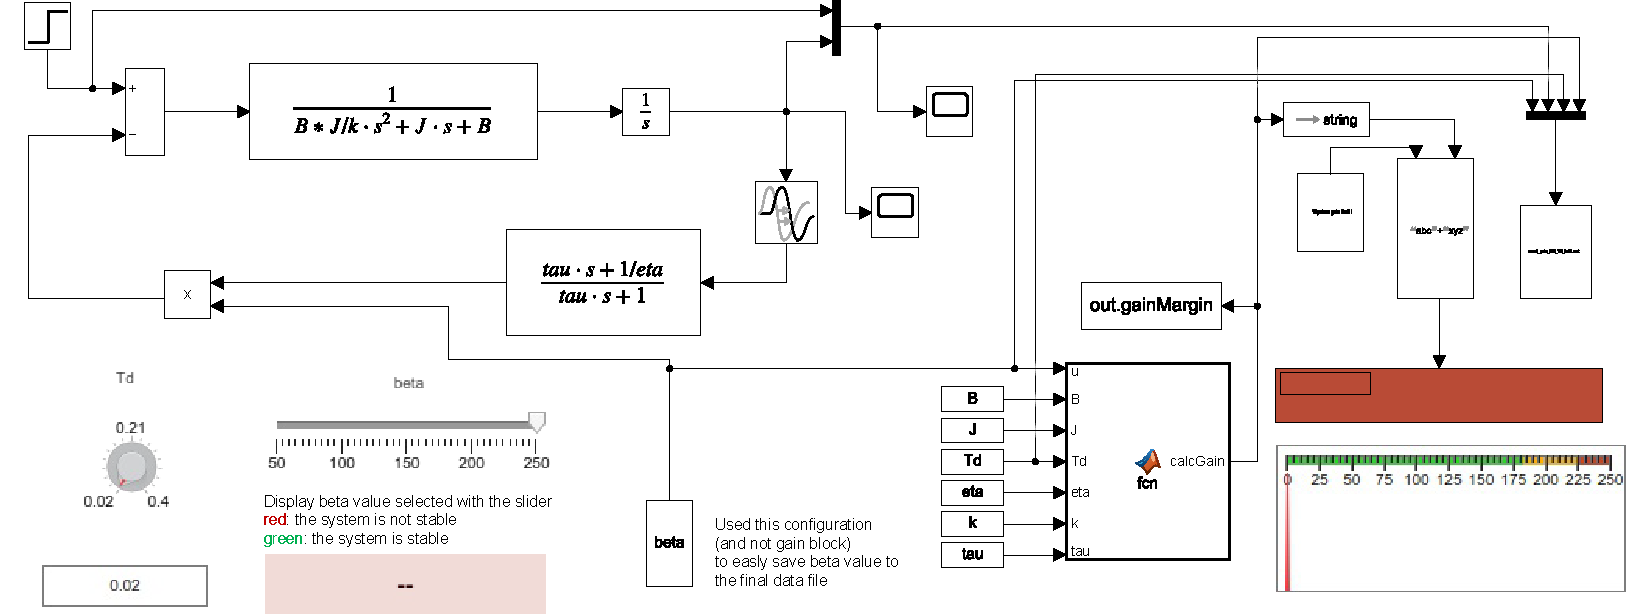
\includegraphics[width=0.95\linewidth]{simulink_stretch}
	\caption{Implementazione Simulink del modello di riflesso muscolare. Il riflesso è implementato nella parte sinistra, le dashboard in basso a sinistra servono a variare i parametri \texttt{Td} e \texttt{beta} visualizzandone i valori. In particolare, i display diventano verdi/rossi a seconda che il guadagno sia tale da rendere il sistema stabile o meno. La parte di destra serve a salvare i risultati facendo in modo che nel nome del file siano presenti i valori dei parametri modificati.}
	\label{fig:simulink_stretch}
\end{figure*}

\subsection{Simulink}

Simulink \cite{simulink} è un software sviluppato da MathWorks che fornisce un approccio grafico basato su un ambiente di modellazione che permette all’utente di convertire il problema in una rete di blocchi di funzioni matematiche.

Inoltre, tale ambiente permette l’integrazione con il linguaggio Matlab e le relative funzioni di programmazione.

Tramite Simulink è possibile implementare i modelli considerati aggiungendo diverse features, quali delle dashboard per interagire con i parametri del sistema, utili ad analizzarne il comportamento e la stabilità.

\section{Risultati}

Tali modelli sono stati implementati all'interno di Simulink analizzandone la stabilità e l'influenza dei diversi coefficienti, in particolare del guadagno.



\begin{figure}[t!]
	\centering
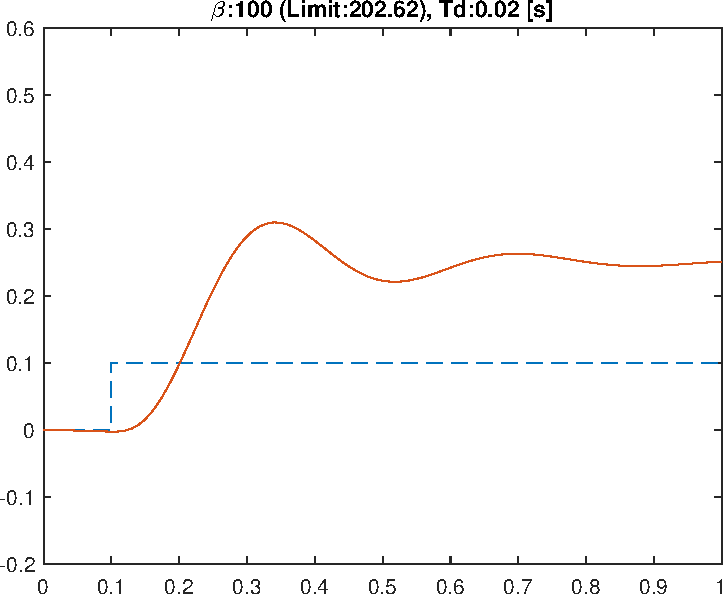
\includegraphics[width=0.95\linewidth]{../code/stretch/figs/result_gain_100_Td_0.02}
\caption{Andamento della risposta al gradino del sistema del riflesso da stiramento. Il sistema, dopo una breve oscillazione iniziale, si porta verso lo stato di equilibrio rimanendo stabile e costante. L'ampiezza del gradino è stata ridotta ed il grafico è utile ad identificare l'instante iniziale.}
\label{fig:beta100}
\end{figure}

\begin{figure*}[t!]
	\begin{subfigure}{0.33\linewidth}
	\centering
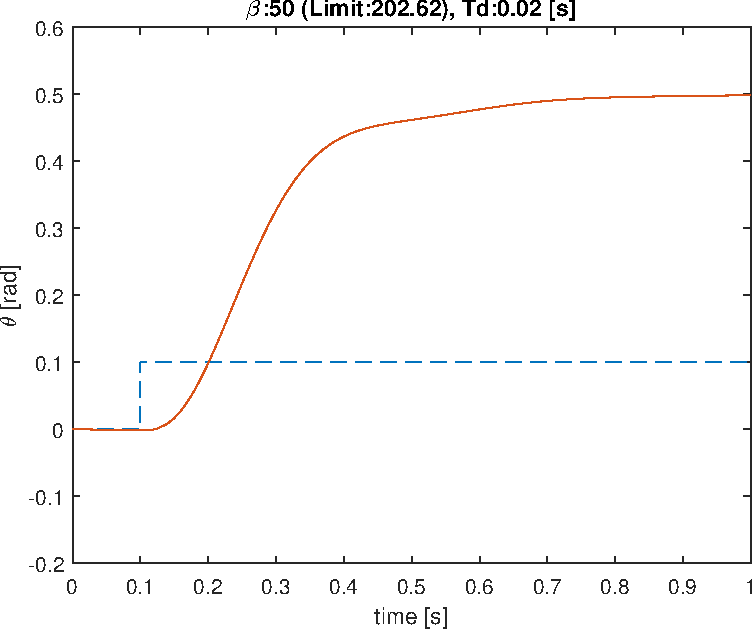
\includegraphics[width=0.95\linewidth]{../code/stretch/figs/result_gain_50_Td_0.02}
\caption{}
	\end{subfigure}\hfill
	\begin{subfigure}{0.33\linewidth}
	\centering
	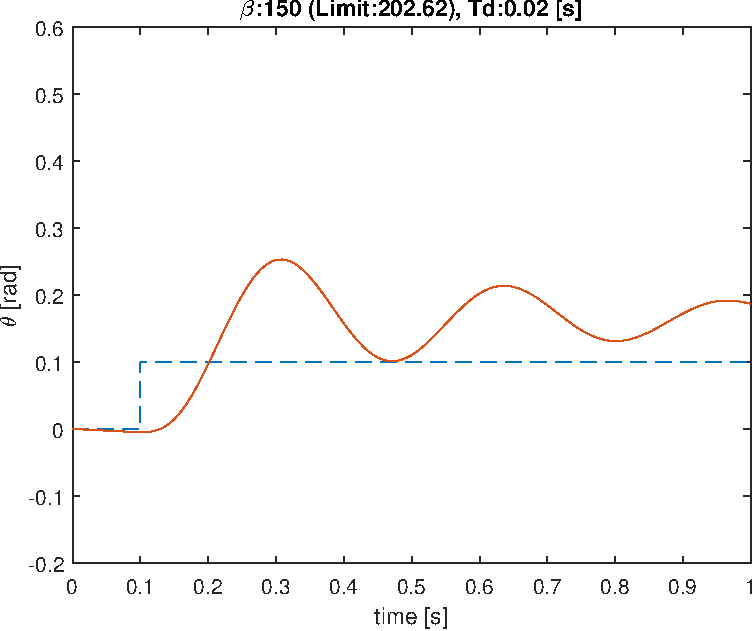
\includegraphics[width=0.95\linewidth]{../code/stretch/figs/result_gain_150_Td_0.02}
	\caption{}
\end{subfigure}\hfill
	\begin{subfigure}{0.33\linewidth}
	\centering
	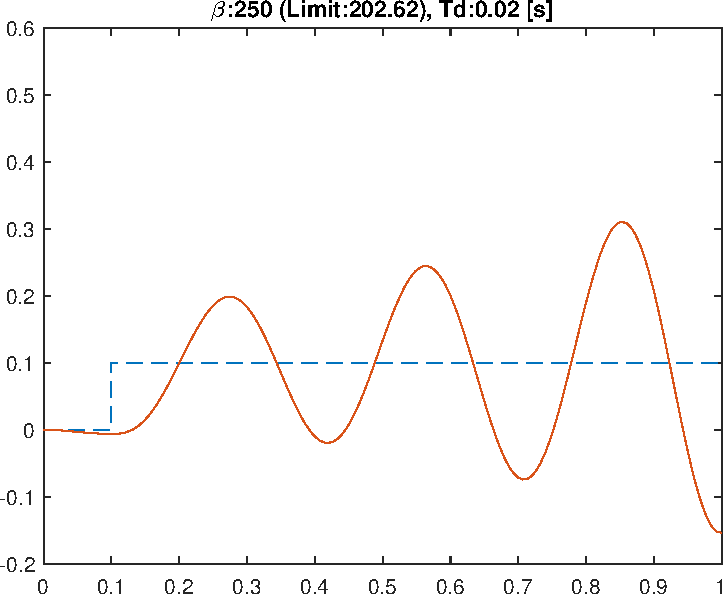
\includegraphics[width=0.95\linewidth]{../code/stretch/figs/result_gain_250_Td_0.02}
	\caption{}
\end{subfigure}\hfill
	\caption{Variazione della risposta del sistema al variare del guadagno. $\beta =50$ (a); $\beta =150$ (b); $\beta=250$ (c). Si vede come all'aumentare del guadagno si riduce l'angolo di equilibrio ma la risposta diventa oscillatore finoa a divergere (instabilità).}
	\vspace{0.5cm}
	\begin{subfigure}{0.5\linewidth}
		\centering
		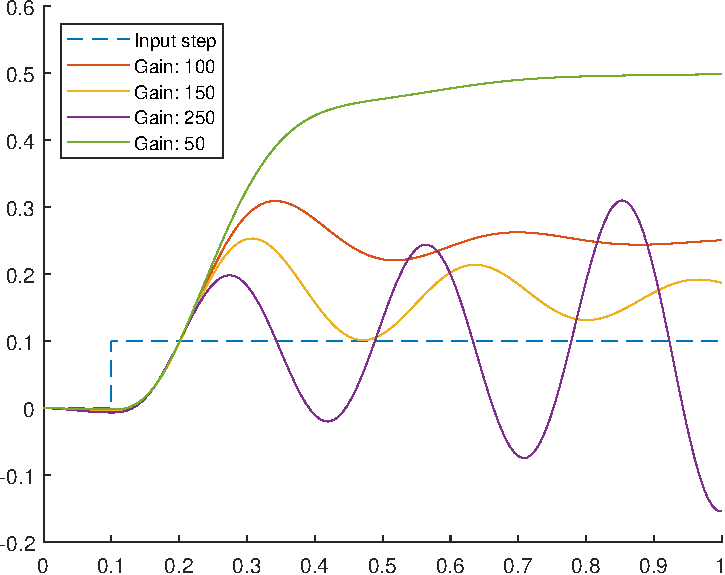
\includegraphics[width=0.85\linewidth]{../code/stretch/figs/gainPlot}
		\caption{}
		\label{fig:stretchGain}
	\end{subfigure}\hfill
	\begin{subfigure}{0.5\linewidth}
		\centering
		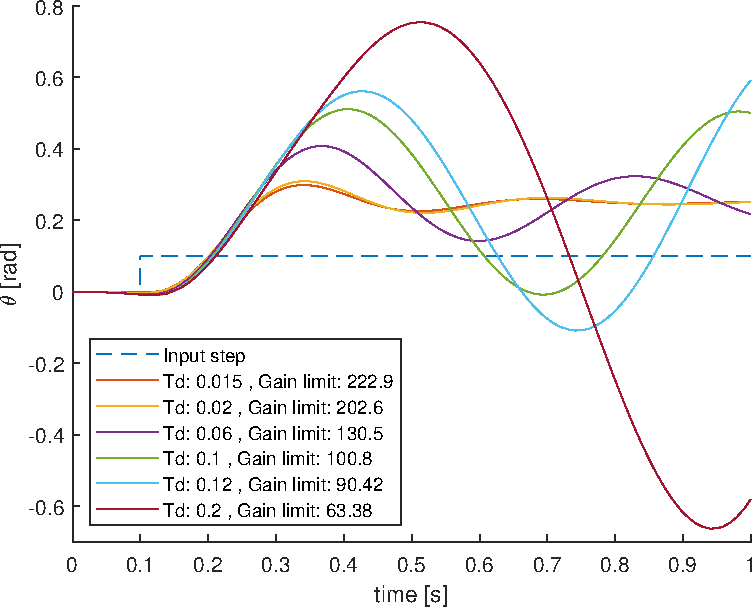
\includegraphics[width=0.85\linewidth]{../code/stretch/figs/TdPlot}
		\caption{}
		\label{fig:stretch_td}
	\end{subfigure}\hfill
	\caption{Confronto della risposta al variare del guadagno (a) o del delay (b). Si vede come al crescere del guadagno la risposta diventa oscillatore pur riducendosi il valore dell'angolo di equilibrio. Al crescere del tempo di ritardo aumenta il tempo necessario a raggiungere l'equilibrio e si abbassa il valore limite di guadagno, quindi è possibile che, a parità di valore di $\beta$ aumentando $T_d$ il sistema diventi instabile.}
		\vspace{0.5cm}
	\begin{subfigure}{0.5\linewidth}
		\centering
		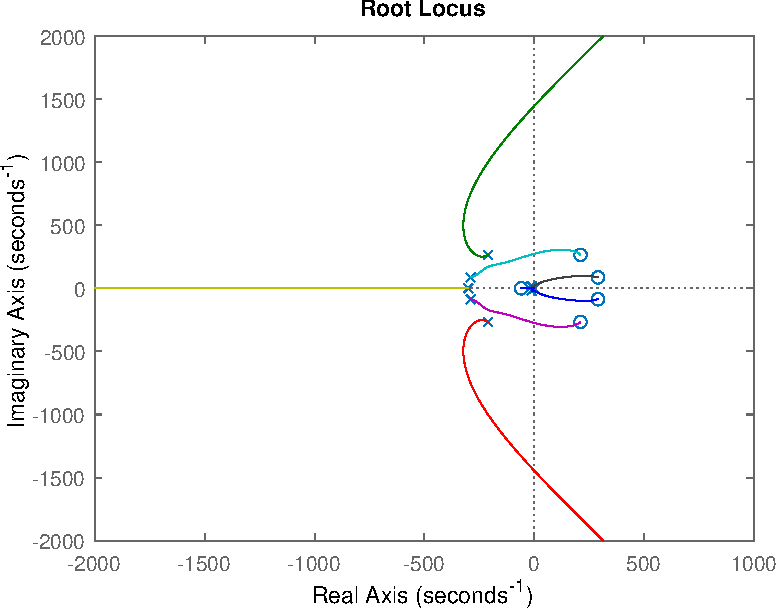
\includegraphics[width=0.85\linewidth]{../code/stretch/figs/rootlocus}
		\caption{}
		\label{fig:rootlocus_stretch}
	\end{subfigure}\hfill
	\begin{subfigure}{0.5\linewidth}
		\centering
		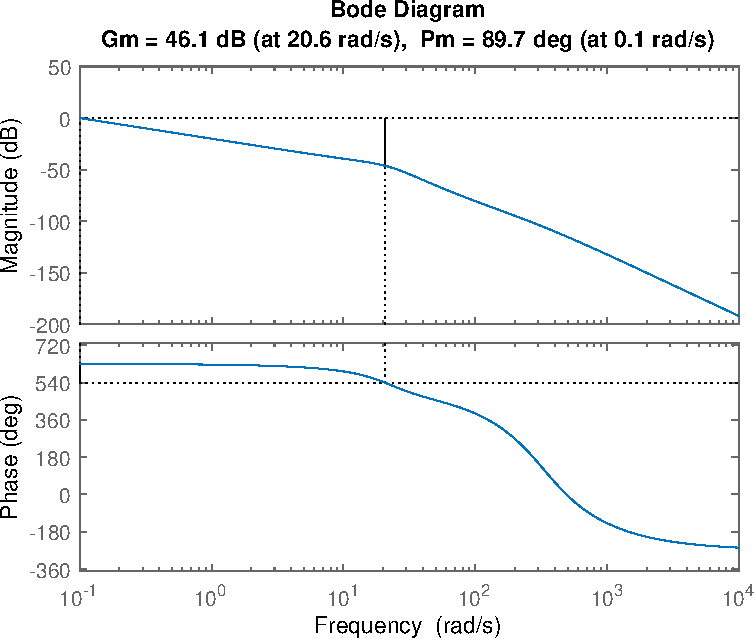
\includegraphics[width=0.85\linewidth]{../code/stretch/figs/margin}
		\caption{}
		\label{fig:margin_stretch}
	\end{subfigure}\hfill
	\caption{Analisi di stabilità con luogo delle radici (a) e margini di guadagno (b). Si vede come il valore limite di $\beta$ con $T_d$ standard e approssimazione di Pade è di 202.62, pari a 46.1 dB.}
	\end{figure*}

\subsection{Riflesso neuromuscolare}

\begin{figure*}[t!]
	\centering
	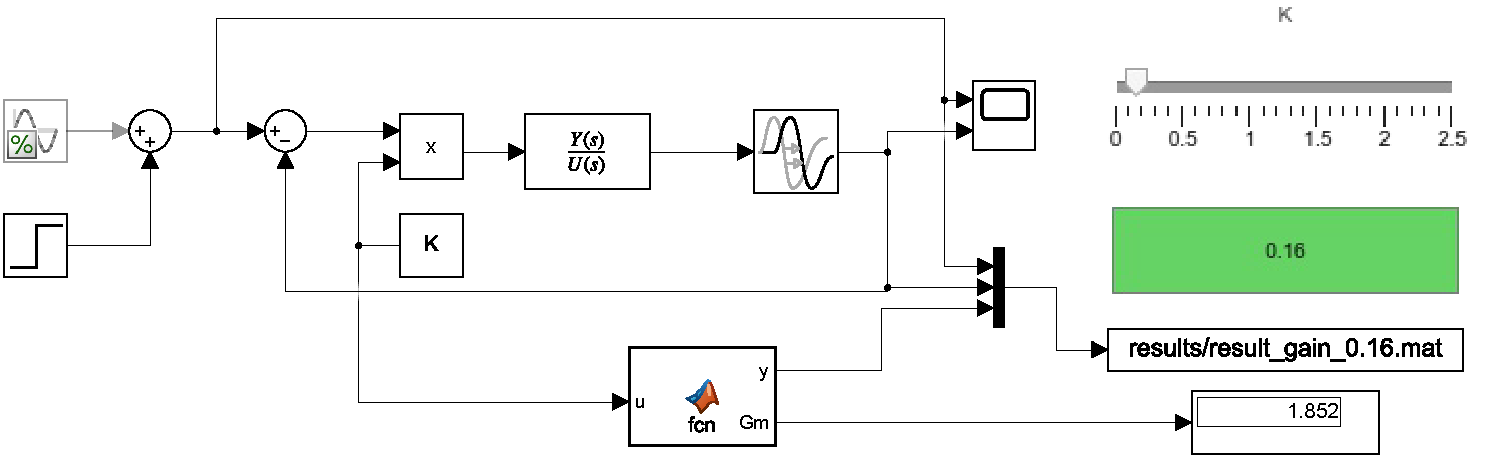
\includegraphics[width=0.8\linewidth]{figures/simulink_pupillary}
	\caption{Modello Simulink del riflesso pupillare dove sono presenti gli ingressi, il sistema di controllo, il blocco \texttt{fcn}, uno slider per regolare il guadagno e relativo display interattivo, il blocco di output e un display per visualizzare il guadagno limite, pari a 1.852. Il display si colora di verde se $K<K_{lim}$ o di rosso se il sistema risulta instabile.}
	\label{fig:simulinkpupillary}
\end{figure*}

\begin{figure*}[t!]
	\begin{subfigure}{0.33\linewidth}
		\centering
		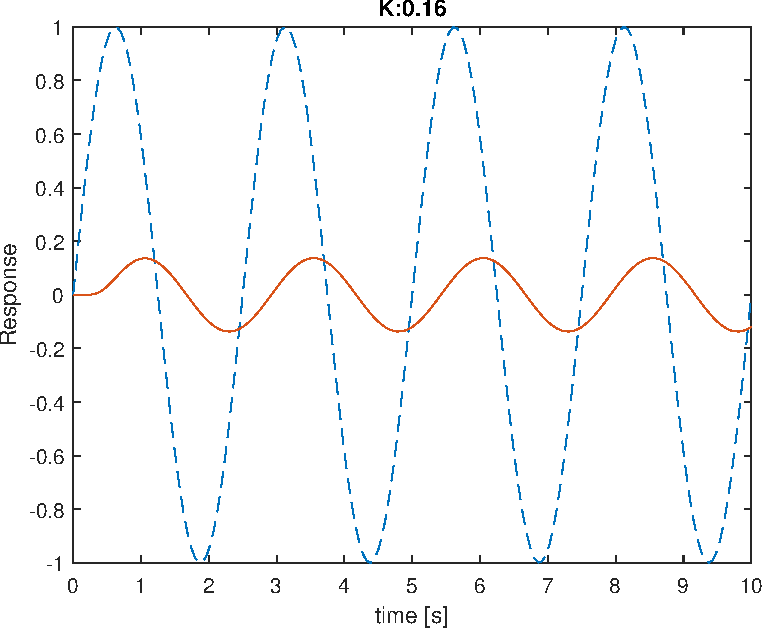
\includegraphics[width=0.95\linewidth]{../code/pupillary/sine/figs/result_gain_0.16}
		\caption{}
	\end{subfigure}\hfill
	\begin{subfigure}{0.33\linewidth}
		\centering
		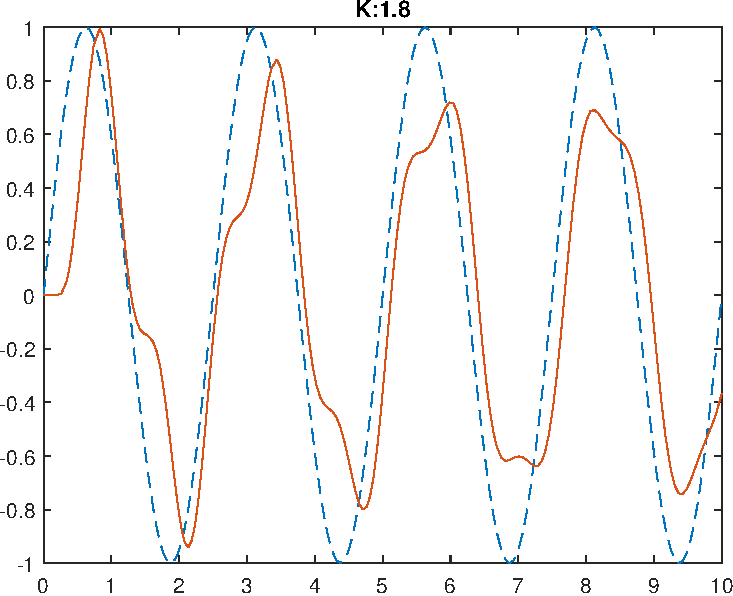
\includegraphics[width=0.95\linewidth]{../code/pupillary/sine/figs/result_gain_1.8}
		\caption{}
	\end{subfigure}\hfill
	\begin{subfigure}{0.33\linewidth}
		\centering
		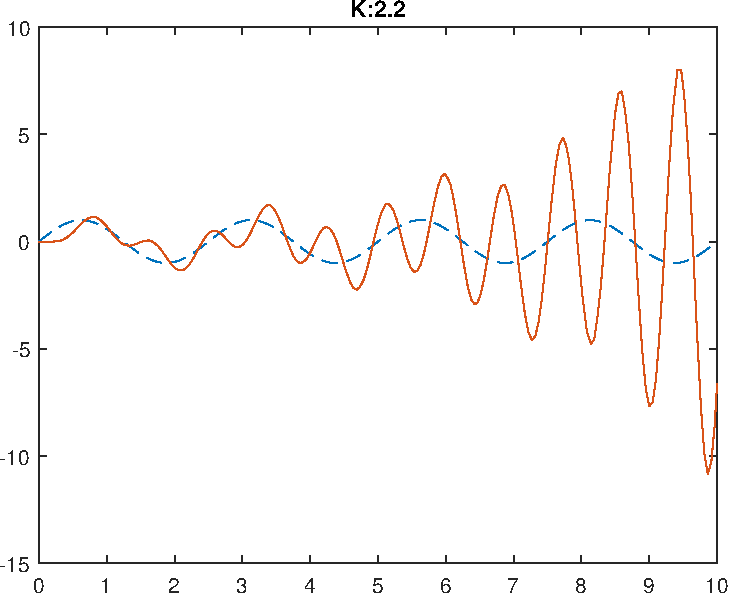
\includegraphics[width=0.95\linewidth]{../code/pupillary/sine/figs/result_gain_2.2}
		\caption{}
	\end{subfigure}\hfill
	\caption{Risposta del sistema di controllo del riflesso pupillare con ingresso sinusoidale al variare del guadagno $K$ con step di default $K=0.16$ (a); $K=1.8$ (b) e sopra il valore limite $K=2.2$ (c). Mentre la risposta in (a) oscilla seguendo il valore di ingresso, pur con un certo sfasamento, l'oscillazione diventa distorta quando $K$ si avvicina al valore limite di $K_{lim}=1.852$ fino a risultare divergente, ed instabile, per valori superiori (c).}
\end{figure*}

Il modello Simulink del riflesso da stiramento è rappresentato in \cref{fig:simulink_stretch} dove, oltre al modello già descritto nello schema a blocchi in \cref{fig:sistemamuscolo} sono presenti alcuni blocchi grafici per cambiare le variabili in gioco e per salvare i dati. In particolare, il blocco \texttt{fnc} viene descritto in appendice (\cref{sec:fcn}).

Il sistema viene analizzato su un tempo da 0 a 1 s osservandone la risposta al gradino dopo 0.1 s. L'andamento del segnale è presente in \cref{fig:beta100}.

Il sistema si porta verso lo stato di equilibrio rimanendo stabile e costante. Inizialmente è presente una leggera oscillazione, intorno il valore di equilibrio, dovuta proprio al guadagno del sistema che tende a compensare il carico aggiunto all'improvviso. 

Tale effetto oscillatorio cresce al crescere del guadagno, come indicato in \cref{fig:stretchGain}.
In particolare, per un guadagno più basso ($\beta =50$) il sistema smette di oscillare ma tende ad equilibrarsi ad un angolo molto maggiore, fino a circa 30° rispetto la configurazione iniziale che ricordiamo essere con il gomito non propriamente perpendicolare ma con un angolo di circa 135°.

Tale sottosmorzamento non è presente per guadagni più alti dove l'angolo di equilibrio diventa molto più basso ma la risposta inizia a diventare oscillatoria. In particolare, per un guadagno di 250 la risposta inizia a divergere e il sistema risulta instabile. 

In particolare, dall'analisi di stabilità si identifica il guadagno limite a 202,62. Tale valore viene identificato considerando l'espansione di Padè per l'esponenziale è analizzandole il luogo delle radici (\cref{fig:rootlocus_stretch}) o tramite il comando Matlab \texttt{margin()} che restituisce il diagramma di Bode e il guadagno limite (\cref{fig:margin_stretch})

Infine, un'ulteriore analisi (\cref{fig:stretch_td}) mostra come al crescere del delay della risposta si riduce il valore del guadagno limite. Per cui ne risulta che, fissando $\beta$ tra le diverse simulazioni al valore di default ($\beta=100$) il sistema risulterà instabile per delay superiori a 0.1. 




\subsection{Riflesso pupillare}

Per analizzare la risposta del riflesso pupillare viene considerata un'onda sinusoidale di frequenza $f=2\pi *0.7 \text{ [rad] }= 0.7 \text{ Hz}$ \cite{stark_servoanalytic_1957}. 
L'analisi viene condotta da 0 a 10 s, analizzando la risposta in termini di dilatazione pupillare. 

Il modello Simulik è presente in \cref{labelfig:simulinkpupillary}. Oltre al diagramma a blocchi precedente illustrato (\cref{fig:pupillary_block}) sono presenti due ingressi, sinusoidale e step, utilizzati singolarmente (commentando o l'uno o l'altro), il blocc \texttt{fcn} analogo al caso del riflesso da stiramento e descritto in \cref{sec:fcn}, uno \texttt{scope} per visualizzare gli andamenti e il blocco per salvare i dati.




\begin{figure*}[t!]
	\begin{subfigure}{0.5\linewidth}
		\centering
		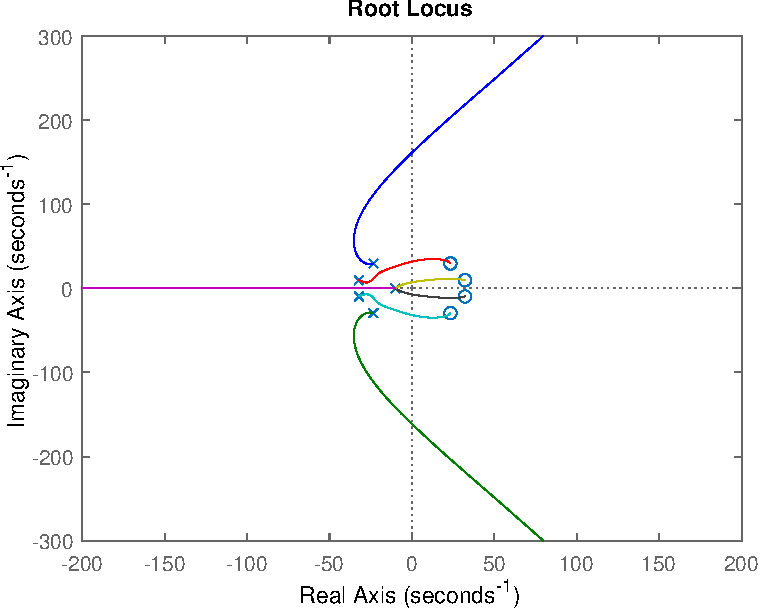
\includegraphics[width=0.9\linewidth]{../code/pupillary/sine/figs/rlocus}
		\caption{}
	\end{subfigure}\hfill
	\begin{subfigure}{0.5\linewidth}
		\centering
		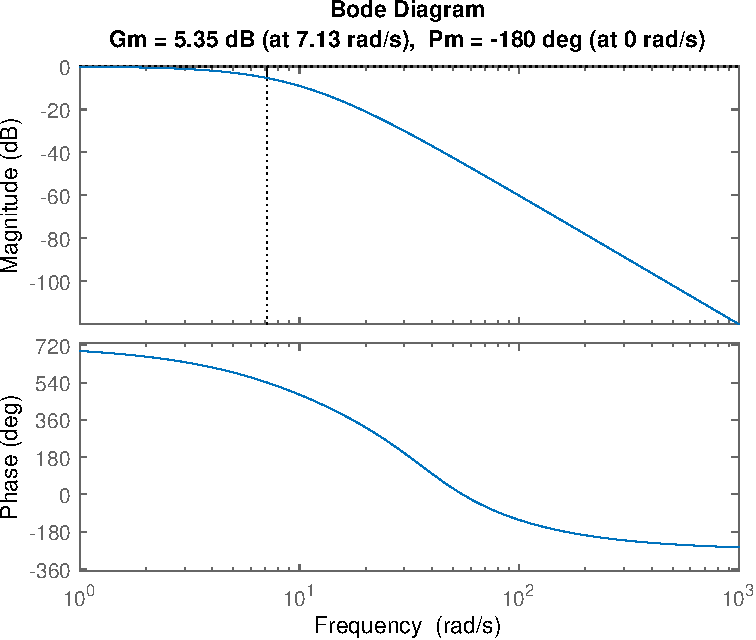
\includegraphics[width=0.9\linewidth]{../code/pupillary/sine/figs/margin}
		\caption{}
	\end{subfigure}\hfill
	\caption{Analisi di stabilità tramite il luogo delle radici (a) e diagramma di Bode (b). Ne risulta un guadagno limite di $K_{lim}=1.852$ pari a 5.32 dB.}
	\label{fig:pup_stabilit}
\end{figure*}

\begin{figure*}[t!]
	\begin{subfigure}{0.5\linewidth}
		\centering
		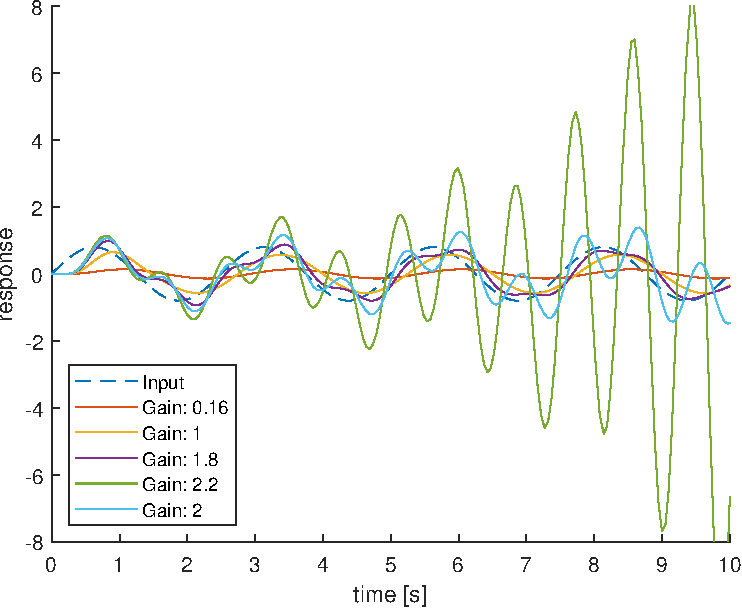
\includegraphics[width=0.9\linewidth]{../code/pupillary/sine/figs/gainPlot}
		\caption{}
		\label{fig:pup_gain}
	\end{subfigure}\hfill
	\begin{subfigure}{0.5\linewidth}
		\centering
		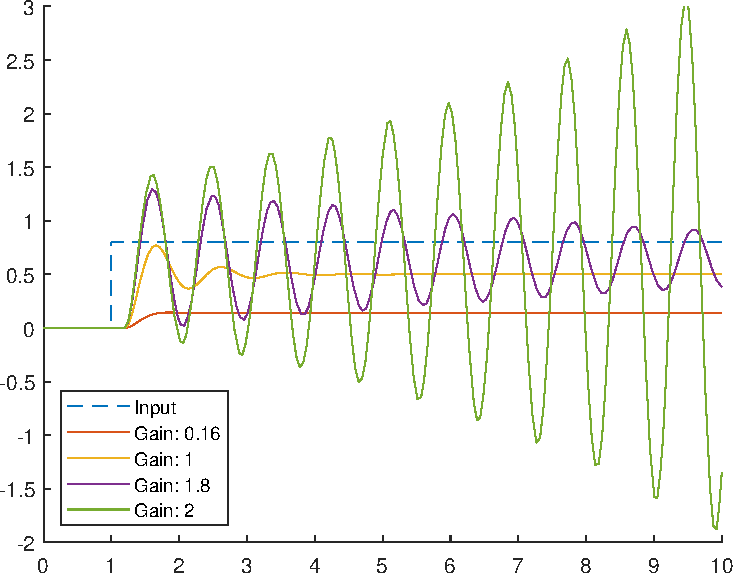
\includegraphics[width=0.9\linewidth]{../code/pupillary/step/figs/gainPlot}
		\caption{}
		\label{fig:pup_step}
	\end{subfigure}\hfill
	\caption{Confronto della risposta al variare del guadagno per ingresso sinusoidale (a) e a gradino (b). Si vede come per valori di $K$ superiori a $K_{lim}=1.852$ il sistema risulta instabile e la risposta diverge.}
\end{figure*}

Ad ingresso sinusoidale corrisponde un'analoga risposta che, per valori di guadagno sufficientemente bassi, insegue l'ingresso con un'oscillazione analoga, seppur sfasata.
Tale oscillazione risente di un effetto di distorsione per valori del guadagno vicini al valore limite fino a risultare instabile e divergente per valori superiori al valore limite. In particolare, in \cref{fig:pup_gain}, vengono confrontati 5 differenti valori di $K$ e le risposte risultanti dallo stesso ingresso. 

Inoltre, è possibile osservare come l'oscillazione instabile risulta a frequenza nettamente maggiore di quella dell'ingresso. 

Il valore limite di guadagno è pari a $K_{lim}=1.852$ ed è stato identificato con un'analisi di stabilità tramite il luogo delle radici in \cref{fig:pup_stabilit}.

Inoltre, si è fatto anche una serie di analisi con ingresso a gradino per analizzare meglio la risposta del sistema e la sua natura oscillatoria. 

Trascurando il valore di default del guadagno, per il quale la risposta risulta stabile e priva di oscillazioni, per i valori analizzati in \cref{fig:pup_step}, la risposta oscilla. Tale oscillazione risulta smorzata o divergente a seconda che il guadagno sia inferiore o superiore al valore limite.

Analizzando la frequenza di oscillazione ($\in [0.8;\:1.1]$ Hz) questa risulta simile ai valori tipicamente indicati in letteratura per il fenomeno dell'hippus \cite{turnbull_origins_2017} e anche alla frequenza critica del sistema (7.13 rad/s).

L'hippus è un particolare fenomeno di movimento ritmico di dilatazione e contrazione pupillare che si instaura in condizioni patologiche come meningiti acute, epilessia o altre malattie cerebrali. Può quindi essere visto come un eccessivo guadagno del sistema, fino a portarlo in instabilità. 



\section{Conclusioni}

Per sottoporre i meccanismi fisiologico ad un'analisi secondo i criteri classici della teoria dei controlli automatici è necessario ottenere un modello di sistema dinamico sufficientemente accurato e allo stesso tempo sufficientemente semplice in termini di costi computazionali e parametri da stimare rispetto l'organismo di interesse.

L'implementazione di un modello di controllore fisiologico all'interno di un ambiente di simulazione interattivo, quale Simulink, consente di analizzarlo e capire l'effetto dei singoli parametri. 

Inoltre, è possibile sfruttare i criteri classici per l'analisi di stabilità e verificare quali parametri portino in instabilità il sistema simulando differenti condizioni patologiche. 

\raggedbottom
\section*{Disponibilità dei dati}

Il materiale è disponibile alla repository online del progetto: \url{https://github.com/mastroalex/reflex}


\raggedbottom
%\pagebreak
\printbibliography[title=Riferimenti]
%\section*{References}

\clearpage
\onecolumn
\section*{Appendice}

Segue la descrizione di due parti importanti per l'implementazione del modello e la produzione dei grafici.

\subsection{Blocco \texttt{fcn}}
\label{sec:fcn}

Entrambi i modelli sfruttando il blocco \texttt{fcn} per automatizzare alcune funzionalità. 

In particolare tale blocco funzione calcola il guadagno limite e lo confronta con il guadagno attuale (settato tramite le dashboard). A seconda che sia maggiore o minore colora di display di rosso e verde. Per poterlo fare, a differenza di Matlab classico, è necessario dichiarare le funzioni come estrinseche ed inizializzare le nuove variabili, dichiarandone anche la classe.

Inoltre, il blocco permette anche di regolare i range dello slider colorato dividendolo in tre regioni (verde, arancio e rosso) e aggiornarlo ad ogni simulazione.

\begin{figure}[h!]
\begin{lstlisting}[language=matlab,style=mystyle]
function [calcGain,u]=fcn(u,B,J,Td,eta,k,tau)
	% this avoid problem with function and code generation
	coder.extrinsic('pade'); coder.extrinsic('tf'); coder.extrinsic('rlocus')
	coder.extrinsic('tf'); 	coder.extrinsic('margin'); coder.extrinsic('type')
	coder.extrinsic('strcat'); 	coder.extrinsic('get_param'); 	coder.extrinsic('set_param')
	% setup color as strings
	green='[ 0.2471    0.7804    0.2392]'; 	red='[0.7255    0.2941    0.2100]';	
	% set trasfer function
	G_num=1;
	G_den=[B*J/k J B];
	int=[1 0];
	F_num=[tau 1/eta];
	F_den=[tau 1];
	% calc pade for numerator exponential expression
	[expon_num_pade,expon_den_pade]  = pade(Td,4);
	% calc transfer function
	num=conv(expon_num_pade,conv(G_num,F_num));
	den=conv(expon_den_pade,conv(int,conv(G_den, F_den)));
	sys=tf(num,den);
	% calc gain margin
	% new varaibles need to be initialized also with class type
	Gm_pade=double(0); 	Gm_pade=margin(sys);
	if u>Gm_pade
		set_param('stretch_reflex/Display1','BackgroundColor',red);
		set_param('stretch_reflex/Display','BackgroundColor',red);
	else
		set_param('stretch_reflex/Display','BackgroundColor',green);
		set_param('stretch_reflex/Display1','BackgroundColor',green);
	end
	% set parameters for the Linear Gauge
	% need struct array like 3x1
	% range.Min with 3x1 minimum, range.Max with 3x1 maximum,  range.Color with [r g b] color
	range=struct('Min',{0; 0.9*Gm_pade; 1.1*Gm_pade},'Max',{0.9*Gm_pade; 1.1*Gm_pade; 250},'Color',{[0.2471  0.7804 0.2392];[0.9294 0.6941 0.1255]; [0.7255 0.2941 0.2000]});
	set_param('stretch_reflex/Linear Gauge','ScaleColors',range)
	calcGain=Gm_pade;
end
\end{lstlisting}
\end{figure}

\subsection{Output}

Il blocco fa anche da \textit{pass trough} per la variabile \texttt{u} ovvero il guadagno attuale così che questo possa essere salvato, a fine simulazione, nel blocco risultati, senza dover aspettare l'aggiornamento delle variabili (che avverrebbe alla simulazione successiva).

Il blocco di output viene rinominato di simulazione in simulazione tramite una funzione di callback, propria del modello, che si attiva ogni volta che viene inizializzata la simulazione. Tramite funzione di callback fa si che il file venga salvato nella cartella \texttt{../results/} e che il nome contenga la concatenazione del nome del parametro e del suo valore, ad esempio:

\begin{equation*}
	\mathtt{results/}+\mathtt{gain}+\{\mathtt{gain}+\}+\mathtt{Td}+\{\mathtt{Td}+\}+\mathtt{.mat}
\end{equation*}

I risultati sono salvati come Timeseries.

\subsection{Plot}

All'interno dei risultati sono presenti, oltre l'input e la risposta, anche i valori dei parametri. Questi vengono utilizzati per le legende e i titoli dei grafici andando a caricare, file per file, una struttura \texttt{data{}} con i seguenti campi:

\begin{figure}[h!]
\begin{lstlisting}[language=matlab,style=mystyle]
file_struct=dir('results/*.mat');
% load all the files in data{} structure with different fields
VAR={};
for i=1:length(file_struct)
	load(strcat('results/',file_struct(i).name))
	data{i}.Time=stretch_reflex_result.Time;
	% use mode() function to avoid numerical error
	% this data have to be consant)
	data{i}.Gain=mode(stretch_reflex_result.Data(:,1));
	data{i}.input=stretch_reflex_result.Data(:,2);
	data{i}.response=stretch_reflex_result.Data(:,3);
	data{i}.Td=mode(stretch_reflex_result.Data(:,4));
	data{i}.margin=mode(stretch_reflex_result.Data(:,5));
	% save the name of the file to export corresponding figs
	data{i}.Name=erase(file_struct(i).name,'.mat');
	clear stretch_reflex_result
end
\end{lstlisting}
\end{figure}


